\begin{frame}{Barjordsstriber}

\small

\begin{columns}[T]

\begin{column}{0.58\textwidth}

\textbf{Regler for barjordsstriber:}

\begin{itemize}[]
\item Udlægges langs søer, vandløb, kystlinjer, vådområder, levende hegn, skovbryn, markskel, diger, fortidsminder, beplantning, vegetationsstriber og naturarealer
\item Min. 1 m bred
\item Min. 50\% soleksponeret
\item Plantedække max. 20\% over 100 m strækning
\end{itemize}

\vspace{0.4em}

\textbf{Gavner arter:}

\footnotesize
Vibe, agerhøne, sanglærke, gul vipstjert, 
rødrygget tornskade, gulspurv, vilde bier, humlebier, dagsommerfugle, 
rovbiller, græshopper, markmus, pindsvin, lækat, musvåge, tårnfalk

\end{column}

\begin{column}{0.40\textwidth}
\centering
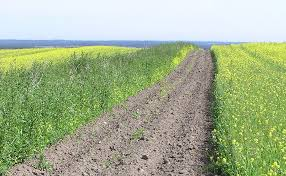
\includegraphics[width=\textwidth]{Billeder/Vildtforvaltning/biotopplantiltag/barjordsstribe.jpeg}
\end{column}

\end{columns}

\end{frame}